    
    %PsyConnect Statistics Guide Source Code
    %Copyright (C) 2022 Ho Han Sheng

    %This program is free software: you can redistribute it and/or modify
    %it under the terms of the GNU General Public License as published by
    %the Free Software Foundation, either version 3 of the License, or
    %(at your option) any later version.

    %This program is distributed in the hope that it will be useful,
    %but WITHOUT ANY WARRANTY; without even the implied warranty of
    %MERCHANTABILITY or FITNESS FOR A PARTICULAR PURPOSE.  See the
    %GNU General Public License for more details.

    %You should have received a copy of the GNU General Public License
    %along with this program.  If not, see <https://www.gnu.org/licenses/>.

    \documentclass[a4paper,11pt]{book}
    \usepackage[T1]{fontenc}
    \usepackage[utf8]{inputenc}
    \usepackage{lmodern}
    \usepackage{hyperref}
    \usepackage{graphicx}
    \usepackage[english]{babel}
    \usepackage{tikz}
    \usepackage{amsmath,amssymb}
    \usepackage{stackengine}
    \usepackage{stix2}
    \usepackage{stix}
    \usepackage{xcolor}
    \usepackage{array}
    \usepackage{tabulary}
    \usepackage{longtable}
    \usepackage{siunitx}
    \usepackage[style=apa]{biblatex}
    \usepackage{csquotes}
    
    
    \addbibresource{bibliography.bib}
    
    \usetikzlibrary{tikzmark,calc,decorations.pathreplacing}
    
    \newcommand\deci[1]{%   <--- Decimal position to right
        \kern-.4ex\stackunder[0.4pt]{$#1$}{$\color{red}\acwunderarcarrow$}
    }
    
    \newcommand\decil[1]{%    <--- Decimal position to left
        \kern-.4ex\stackunder[0.4pt]{$#1$}{%
          \reflectbox{$\color{red}\kern-.6ex\acwunderarcarrow$}
          }
    }
    
    % 'dedication' environment: To add a dedication paragraph at the start of book %
    
    \newenvironment{dedication}
    {
       \cleardoublepage
       \thispagestyle{empty}
       \vspace*{\stretch{1}}
       \hfill\begin{minipage}[t]{0.66\textwidth}
       \raggedright
    }
    {
       \end{minipage}
       \vspace*{\stretch{3}}
       \clearpage
    }
    
    % Book's title and subtitle
    \title{\Huge \textbf{PsyConnect Statistics Guide}  \\ \huge v0.1}
    % Author
    \author{\textsc{\underline{Ho} Han Sheng}\thanks{\url{https://github.com/ho-han-sheng}}}
    \date{published date}
    
    \begin{document}
    
    \frontmatter
    \maketitle
    
    % Dedication page
    \begin{dedication}
    <Dedication page>.
    \end{dedication}
    
    % Auto-generated table of contents, list of figures and list of tables 
    \tableofcontents
    \listoffigures
    \listoftables
    
    \mainmatter
    
    % Preface %
    \chapter*{Preface}
    A common aversion faced by psychology undergraduates around the world is the need to study statistics. Given the relative infancy of psychology compared to other hard science fields or even the humanities, it is imperative that we as psychologists are able to read, comprehend and incorporate the most recent research as part of our continuous learning journey. With strong statistical foundations, one would be able to discern sound and rigourous statistical analyses from misleading or erroneous methods used in a fair percentage of psychological research \autocite{Bakker2011}. 
    
    In some universities, the compulsory statistics modules are taught by mathematics professors. This is logical given their area of expertise but may further exacerbate the "expert blind spot" effect \autocite{Nathan2003}. As experts, professors perform many abstract and symbolic reasoning steps automatically, "jumping" from one train of thought to another seamlessly as they would perceive. However, as undergraduates attempting to learn these concepts from scratch, it is exceptionally difficult to be able to "see" these connections automatically or even at all. Additionally, as psychology majors, certain "mathematical connections" inculcated in students majoring in fields requiring substantial mathematical foundations (e.g. engineering, computer science, mathematics) would be difficult to develop in short duration. What professors feel is trivial and does not require explicit instruction then, is what leads to students falling through the cracks. 
    
    In the case of my university (Singapore University of Social Sciences), the psychology program is fully part-time. The typical student profile then consists of mid-career switchers, mature adults and others who have gone years since their last interaction with mathematics. Assuming one leaves the education system with a GCE "O" Levels at 16 years old and pursues a non-mathematically heavy diploma in a polytechnic, it would be 6 years (!) before one can enrol in a part-time course with 2 years of working experience at 22 years old. That is akin to spending 6 years in a sedentary lifestyle with minimal exercise, making it difficult to return to a certain level of fitness. 
    
    \section*{What this book is for}
    This book then serves to hopefully bridge this gap between expert knowledge and novice learning. Content will first focus on topics expected of students at "O" Levels, following the syllabus document published by the Singapore Examinations and Assessment Board. Afterwards, topics related to or typically required to understand statistical concepts at the undergraduate level will be discussed. 
    
    By attempting to keep technical jargon to a minimum, this book should require minimal effort to comprehend concepts. It would also provide a sort of "warm-up" for students' minds to prepare them to think mathematically, serving as pre-reading before they embark on their statistics modules.
    
    
    \section*{What this book is for me}
    My handwriting is terrible. When I first started my statistics modules, I needed a way to write my notes such that they were at least legible and easily written (i.e. typed out because I'm lazy). I was already using Notion to develop my own notes for my psychology modules and a quick google bestowed upon me the masterpiece that is \LaTeX{}. Notion allowed me to typeset mathematical formulae with \LaTeX{} commands and what followed was the development of my summary notes that were shared to my fellow psychology peers. 
    
    This book is then a personal project for me to further develop my skills in working with \LaTeX{}, from typesetting everything within the document, learning the uses of various packages (\textsc{TikZ}, \textsc{tabulary}, \textsc{Bib}\LaTeX{} etc.) to creating my own graphics and figures in \LaTeX{}.
    
    
    % Short description of each chapter
    \section*{Structure of book}
    
    Each unit will focus on <SOMETHING>.
    
    \section*{About the companion website}
    The website\footnote{\url{<insert github link>}} for this file contains:
    \begin{itemize}
      \item The (freely downlodable) latest version of this document.
      \item The LaTeX source code for this document.
      \item Miscellaneous material
    \end{itemize}
    
    
    \section*{Acknowledgements}
    \begin{itemize}
    \item A special word of thanks goes to  
    
    \end{itemize}
    \mbox{}\\
    %\mbox{}\\
    \noindent Ho Han Sheng \\
    \noindent \url{https://github.com/ho-han-sheng/}
    
    
    % Start actual book content
    \chapter{Numbers and Algebra}
    
    \section{Numbers and their operations}
    
    \subsection{Number systems}
    
    What do these funny looking letters $\mathbb{R}$, $\mathbb{N}$, $\mathbb{Z}$, $\mathbb{Q}$ mean? These symbols denote which sets a particular number falls under (real, natural, integer etc.). Later on we will look at how these symbols may be used in set theory. Table \ref{tab:Number set notations} on page \pageref{tab:Number set notations} outlines the main terms used. 
    
    \begin{table}[p]
        \centering
        \settowidth\tymin{{Example} + 5pt}
        \setlength\extrarowheight{4pt}
            \begin{tabulary}{\linewidth}{|L|C|J|C|}
                \hline
                \textbf{Set} & \textbf{Symbol} & \textbf{Definition} & \textbf{Example} \\
                \hline \hline
                Natural numbers & $\mathbb{N}$ & Also called counting numbers, these are numbers we use to count items & $1, 2, 3, 4, 5$, \ldots \\
                \hline
                Whole numbers & No official symbol & Includes the set of natural numbers and $0$ & $0, 1, 2, 3, 4, 5$, \ldots \\
                \hline
                Integers & $\mathbb{Z}$ & Consists of whole numbers, their opposites and $0$ & \ldots $,-3, -2, -1,$ $0, 1, 2, 3$, \ldots \\
                \hline
                Rational numbers & $\mathbb{Q}$ & All numbers that can be expressed as a fraction & $44, -\frac{17}{5},$ $0.1\dot{2} = \frac{11}{90}$ \\
                \hline
                Irrational numbers & No official symbol & Numbers that cannot be expressed as a fraction & $\pi, \sqrt{2}, -3\pi,$ Euler's number \\
                \hline
                Real numbers & $\mathbb{R}$ & Encompasses all rational and irrational numbers. Every number that can exist on a typical number line & \ldots $, -5, -\pi, 0,$ $\sqrt{17}, 75$\\
                \hline
                Imaginary numbers & No official symbol & Any real number multiplied by $\sqrt{-1} = i$ & $2i, \pi i, -3i$ \\
                \hline
                Complex numbers & $\mathbb{C}$ & Includes the set of real numbers. Any number that has a real part and imaginary part. & $(2+3i), (\pi - 6i)$ \\
                \hline
            \end{tabulary}
        \caption{Number set notations}
        \label{tab:Number set notations}
    \end{table}
    
    \subsection{Less than, greater than or equal to}
    Also called inequality symbols, they are used to represent the relationship between two variables or expressions.
    \medskip
    
    \par The value of \(a\) is less than the value of \(b\):
    \[a < b\]
    
    
    The value of \(a\) is greater than the value of \(b\):
    \[a > b\]
    
    
    The value of \(a\) is less than or equal to the value of \(b\):
    \[a\leq b\]
    
    
    The value of \(a\) is greater than or equal to the value of \(b\):
    \[a\geq b\]
    
    \noindent\textbf{Useful Tip:} Imagine the inequality symbol as a crocodile's mouth and that the crocodile prefers eating larger numbers.
    
    \subsection{Approximation and estimation}
    Significant figures refer to the number of digits in a value that are necessary and contribute to the degree of accuracy of the quantity of something. Insufficient significant figures during your calculations can lead to an inaccurate final answer. As a rule of thumb, \emph{five} significant figures are used for intermediate calculations and \emph{three} significant figures are used for your final answer. 
    
    We start by counting the digits from left to right, beginning with the first \emph{non-zero} digit. To round off to \emph{three} significant figures, we have to look at the fourth non-zero digit from the left. 
    
    \[0.0\tikzmark{a}{7}56\tikzmark{e}{9}\]
    
    \[\tikzmark{b}{7}89\tikzmark{f}{0}43.0889\]
    
    \[0.0\tikzmark{c}{4}59\tikzmark{g}{6}0\]
    
    \[\tikzmark{d}{3}00\tikzmark{h}{2}.01\]
    
    \begin{tikzpicture}[remember picture,overlay]
    
    %There's probably a better way to use tikzmarks here but it works so
    % todo align the 1st and 4th labels
    {
    \foreach \Value in {a, b, c, d}
    \draw [<-]
      ([yshift = -2pt, xshift = 3.5pt]pic cs:\Value) node[anchor = south] {} -- ([yshift = -8pt, xshift = 3.5pt]pic cs:\Value) 
      node[anchor=north, inner sep = 0.5pt] {1st};
    
    \foreach \Value in {e, f, g, h}
    \draw [<-]
      ([yshift = -2pt, xshift = 3.5pt]pic cs:\Value) node[anchor = south] {} -- ([yshift = -8pt, xshift = 3.5pt]pic cs:\Value) 
      node[anchor=north, inner sep = 0.5pt] {4th};
    }
    \end{tikzpicture}
    
    The value of this fourth digit determines how we round off the number. If the value of the fourth digit is $\geq5$ then we will add 1 to the third digit. 
    
    % todo align all equations at approx
    
    \[0.075 \tikzmarknode{1a}{6}9 \approx 0.0757\]
    
    \[78 \tikzmarknode{1b}{9}043.0889 \approx 789000\]
    
    \[0.045\tikzmarknode{1c}{9}60 \approx 0.0460\]
    
    \[30\tikzmarknode{1d}{0}2.01 \approx 3000\]
    
    \begin{tikzpicture}[remember picture,overlay]
    
    
    {
    \foreach \Value in {1a, 1c}
    \draw [<-]
      ([yshift = -2pt]pic cs:\Value) node[anchor = south] {} -- ([yshift = -8pt]pic cs:\Value) 
      node[anchor=north, inner sep = 0.5pt] {Add 1};
    
    \foreach \Value in {1b, 1d}
    \draw [<-]
      ([yshift = -2pt]pic cs:\Value) node[anchor = south] {} -- ([yshift = -8pt]pic cs:\Value) 
      node[anchor=north, inner sep = 0.5pt] {Keep value};
    }
    
    \end{tikzpicture}
    
    If the value of the fourth digit is $\leq4$, then we will keep the value of the third digit. Note that the subsequent digits will become 0. For \emph{five} significant figures then, we would look at the sixth non-zero digit from the left.
    
    \pagebreak
    \subsection{Scientific notation}
    Also known as standard form. This is a way to express numbers that are either very large or very small.
    
    \[ A \times 10^n \]
    
    Where $n$ is an integer\footnote{Do you remember what an integer is? Refer back to Table \ref{tab:Number set notations} if you need to.} and $1 \leq A < 10$
    \medskip
    
    The advantage of scientific notation lies in its lack of ambiguity in the number of significant figures. Refer to the number 3000, which is valid for 1, 2, 3 or 4 significant figures. As seen in Table \ref{tab:Decimal and scientific notation}, $3.251 \times 10^{6}$ is clearly 4 significant figures. Some calculators display $\text{\sc{e}}$ in place of $\times 10$. $3.251 \times 10^{6}$ would then appear as $3.251\text{\sc{e}}6$.
    
    \begin{table}[htb]
        \centering
        {\renewcommand{\arraystretch}{1.5}%
        \begin{tabular}{|l|r|}
        \hline
        \textbf{Decimal Notation} & \textbf{Scientific Notation}  \\
        \hline \hline
        3     &   $3 \times 10^{0}$  \\
        \hline
        3000 &   $3 \times 10^{3} $   \\
        \hline
        3251000 & $3.251 \times 10^{6}$   \\
        \hline
        0.02 &  $2 \times 10^{-2}$    \\
        \hline
        0.0000451 & $4.51 \times 10^{-5}$ \\
        \hline
        0.000060075 & $6.0075 \times 10^{-5}$  \\
        \hline
        \end{tabular}}
        \caption{Decimal and scientific notation}
        \label{tab:Decimal and scientific notation}
    \end{table}
    
    \noindent\textbf{Useful Tip:} $n$ can be thought of as the number of times we move the decimal point left or right\footnote{Only applicable for base 10.}. 
    
    \[ 3.251 \times 10^{6} = 3. \underbrace{\deci{2}\deci{5}\deci{1}\deci{0}\deci{0}\deci{0}}_{6 \:\text{places}} = 3251000 \]
    
    \[ 6.0075 \times 10^{-5} = 0\, \underbrace{\decil{0}\decil{0}\deci{0}\decil{0}\decil{6}}_{5 \: \text{places}}.0075 = 0.000060075 \]
    
    \pagebreak
    \subsection{Indices}
    
    An index (Plural: indices) is the small superscript number that appears above a number. It denotes the number of times that number is multiplied by itself. $10^{4}$ means 10 multiplied by itself 4 times, $10 \times 10 \times 10 \times 10 = 10000$. We can read this as "10 to the power of 4" or "10 raised to the power of 4".
    
    \[ \tikzmarknode{base}{a}^{\tikzmarknode{index}{m}} \]
    
    \begin{tikzpicture}[remember picture,overlay]
    \draw[<-] 
      ([shift={(0pt,-2pt)}]pic cs:base) |- ([shift={(-10pt,-10pt)}]pic cs:base) 
      node[anchor=east] {Base}; 
    \draw[<-] 
      ([shift={(2pt,5pt)}]pic cs:index) node[anchor=north] {} |- ([shift={(10pt,14pt)}]pic cs:index) 
      node[anchor=west] {Index}; 
    \end{tikzpicture}
    
    There exists index laws and rules that allow us to simplify expressions when working with indices.
    
    %%todo align all equations 
    
    \begin{equation}\label{eqn:index law one}
        a^m \times a^n = a^{m+n}
    \end{equation}
    
    \[2^4 + 2^3 = 2^{4+3} = 2^7 = 128\]
    
    \emph{\ref{eqn:index law one}}. If 2 numbers with the same base are multiplied together, the result is equal to the same base raise to the power of the sum of the 2 indices. 
    
    \begin{equation}\label{eqn:index law two}
        (a^m)^n = a^{m\times n}
    \end{equation}
    
    \[ (2^4)^3 = 2^{4 \times 3} = 2^{12} = 4096 \]
    
    \emph{\ref{eqn:index law two}}. If a number $a^m$ is itself raised to another power, the result is equal to the same base raised to the power of the 2 indices multiplied together.
    
    \begin{equation}\label{eqn:index law three}
        \frac{a^m}{a^n} = a^{m-n}
    \end{equation}
    
    \[ \frac{2^5}{2^3} = 2^{5-3} = 2^2 = 4\]
    
    \[ \frac{2^5}{2^3} = 2^5/2^3 \]
    
    \emph{\ref{eqn:index law three}}. The result of the division of 2 indices is equal to the same base raised to the power of the subtraction of the denominator's index from the numerator's index. 
    
    \pagebreak
    \begin{equation}\label{eqn:index law four}
        a^{-m} = \frac{1}{a^m}
    \end{equation}
    
    \[ 2^{-3} = \frac{1}{2^3} \]
    
    \emph{\ref{eqn:index law four}}. The result of a number raised to a negative power is equal to the reciprocal\footnote{The reciprocal of $X = \frac{1}{X}$} of the same number raised to a positive number of the same value. 
    
    \begin{equation}\label{eqn:index law five}
        a^0 = 1
    \end{equation}
    
    \[ 2^0 = 381^0 = 0^0 = 1 \]
    
    \emph{\ref{eqn:index law five}}. Any base raised to the power of 0 will always give a value of 1.
    
    \begin{equation}\label{eqn:index law six}
        a^{\frac{m}{n}} = \sqrt[n]{a^m}
    \end{equation}
    
    \[ 4^{\frac{2}{3}} = \sqrt[3]{4^2} \]
    
    \emph{\ref{eqn:index law six}}. If the index is a fraction, the denominator $n$ indicates the $n\text{th}$ root and the numerator indicates the power to raise the base by. 
    
    \begin{equation}\label{eqn:index law seven}
        a^m \times b^m = ab^m
    \end{equation}
    
    \[ 2^3 \times 4^3 = (2 \times 4)^3 = 8^3 = 512 \]
    
    \emph{\ref{eqn:index law seven}}. The result of the multiplication of 2 numbers with different bases but with the same index is equal to the multiple of both bases raised to the same power. 
    
    \begin{equation}\label{eqn:index law eight}
        a^m / b^m = \frac{a^m}{b^m} = \bigg(\frac{a}{b}\bigg)^m
    \end{equation}
    
    \[ \frac{2^5}{3^5} = \bigg(\frac{2}{3}\bigg)^5 = \frac{32}{243} \]
    
    \emph{\ref{eqn:index law eight}}. The division of 2 numbers with different bases but with the same index yields a result equal to the fraction (or division) of the two bases raised to the same power. 
    
    \section{Percentages}
    
    \subsection{Expressing quantities as percentages}
    
    
    
    
    
    
    
    
    
    
    \section{Another section heading}
    Lorem ipsum dolor sit amet, consectetur adipisicing elit, sed do eiusmod tempor incididunt ut labore et dolore magna aliqua. Ut enim ad minim veniam, quis nostrud exercitation ullamco laboris nisi ut aliquip ex ea commodo consequat.
    
    
    
    \printbibliography
    
    \end{document}
    